% Seccion de modelado de la memoria. Autocontenida: se puede compilar sola
% (pdflatex seccion_modelo.tex, dos pasadas) o pegarse dentro de
% BORRADOR_memoria_ML.tex, cuyo preambulo ya trae todos estos paquetes.
% Texto en UTF-8 con tildes; el preambulo carga inputenc/fontenc, asi que
% compila tal cual. Si se pega dentro de BORRADOR_memoria_ML.tex, que hoy esta
% escrito sin tildes, hay que acentuar tambien aquel fichero: no mezclar los
% dos criterios dentro del mismo documento.
% Figuras: figs/  (generadas por figs/scripts/, ver figs/scripts/comun.py)
\documentclass[10pt,a4paper]{article}

\usepackage[T1]{fontenc}
\usepackage[utf8]{inputenc}
\usepackage{lmodern}
\usepackage[margin=2.1cm,top=1.8cm,bottom=1.8cm]{geometry}
\usepackage{graphicx}
\usepackage{booktabs}
\usepackage{array}
\usepackage{caption}
\usepackage{capt-of}
\usepackage{xcolor}
\usepackage{microtype}
\usepackage{amsmath}
\usepackage[hidelinks]{hyperref}

\renewcommand{\tablename}{Tabla}
\renewcommand{\figurename}{Figura}
\graphicspath{{figs/}{figuras/}{../../02_eda/figuras/}}
\captionsetup{font=footnotesize,labelfont=bf,skip=3pt}
\renewcommand{\arraystretch}{1.08}
\setlength{\parskip}{0.25em}
\setlength{\emergencystretch}{3em}
\newcolumntype{L}[1]{>{\raggedright\arraybackslash}p{#1}}
\newcommand{\var}[1]{\texttt{\footnotesize #1}}
% Marcas de revision. Version final: \renewcommand{\marca}[1]{}
\newcommand{\marca}[1]{{\color{red}\footnotesize\textbf{#1}}}

\begin{document}

\section{Modelado predictivo del riesgo diario de incendio}

El componente que se describe aquí contesta una pregunta operativa estrecha: de
las 498.530 celdas de un kilómetro en que queda dividida la España peninsular,
cuáles van a arder hoy. No es una pregunta de susceptibilidad ---qué territorio
es propenso al fuego, que se responde con un mapa fijo--- sino de ordenamiento
dentro de un día concreto. El producto es un ranking diario de celdas y lo único
que importa de él es si las celdas que efectivamente ardieron caen arriba. Esa
distinción, que parece de matiz, resultó ser el eje del trabajo.

Era necesario porque la parte de este TFM que ya estaba en producción ---un
modelo entrenado con un muestreo clásico en la literatura de susceptibilidad---
alcanzaba un AUC-ROC de 0,89 en su propio conjunto de test y caía a 0,56--0,64
cuando se le pedía ese ranking contra superficie quemada real.
La sección documenta por qué ocurre esa caída, qué se descartó antes de dar con
la causa, cómo se rediseñó el conjunto de entrenamiento y cuánto se ganó: dos
iteraciones completas del mismo problema separadas por un diagnóstico, y una
comparación de ambas sobre los mismos días y las mismas fuentes.

El resultado principal, anticipado: la caída no venía del ajuste, ni de la
meteorología, ni del desajuste entre entrenamiento y servicio, sino de la
especificación ---de qué se toma como positivo y, sobre todo, como negativo--- y
corregirla lleva el AUC dentro del día de la temporada 2026 de 0,647 a 0,759,
una diferencia pareada de $+0,112$ con intervalo de confianza al 95\,\%
$[+0,074,\ +0,151]$ sobre 74 días. La figura~\ref{fig:f1} sitúa las dos
iteraciones y el diagnóstico que las separa.

\begin{center}
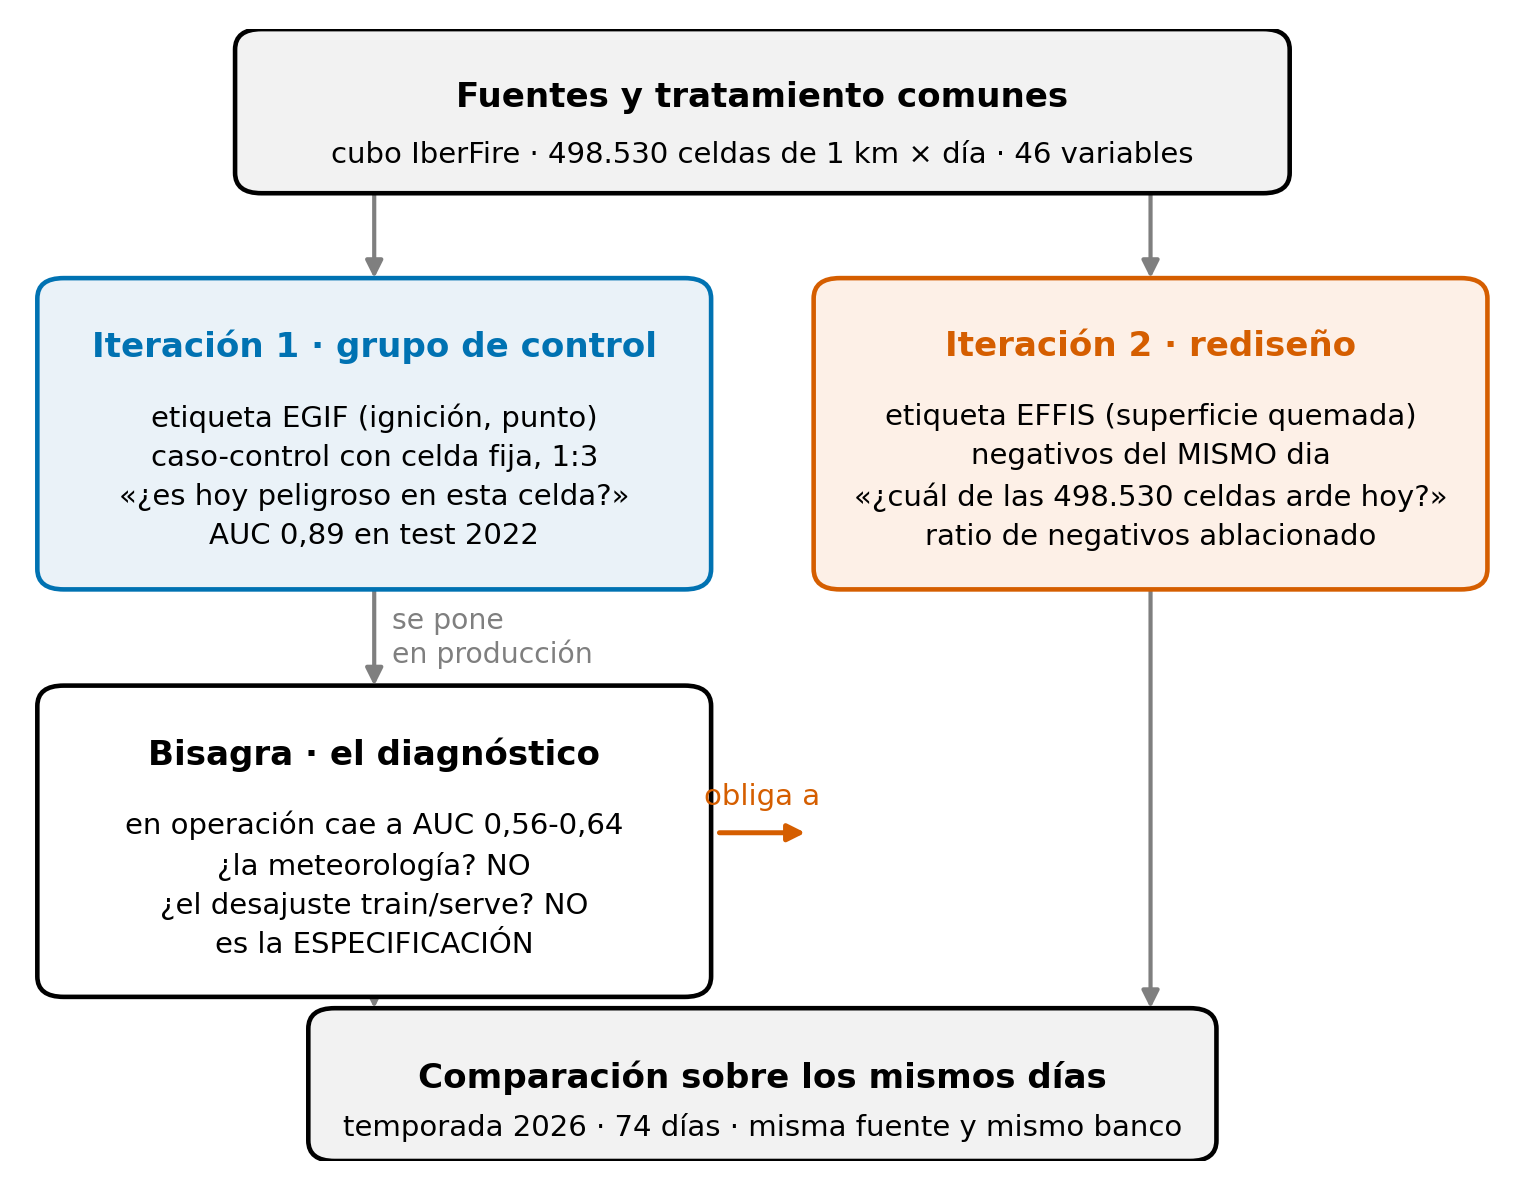
\includegraphics[width=0.84\linewidth]{f1_iteraciones.png}
\captionof{figure}{Las dos iteraciones del trabajo y la bisagra que las separa.
Lo que cambia entre ellas no son las fuentes ni las variables ---son las mismas
46 en las dos--- sino qué se toma como positivo, qué como negativo y contra qué
verdad se valida. La iteración~1 se puso en producción y es el grupo de control
contra el que se mide todo lo demás.}
\label{fig:f1}
\end{center}

\subsection{Datos y preparación}

El soporte del trabajo es IberFire, un datacubo público de riesgo de incendio
para la Península Ibérica: un NetCDF de 30,3\,GB con 261 variables sobre una
malla de 1.188$\times$920 celdas de un kilómetro (EPSG:3035), paso diario y
cobertura 2007--2024. Una fila de entrenamiento es la lectura de todas sus capas
en una celda y un día, y de ahí salen 45 de las 46 variables. Su
meteorología resultó ser el reanálisis ERA5-Land remuestreado (correlaciones de
0,987 a 0,998 y sesgo nulo), con dos discrepancias que condicionan el servicio:
la precipitación viene dividida por un factor de 2,02, y su índice FWI ---el
Fire Weather Index canadiense, la escala meteorológica de peligro de uso
estándar--- solo se reproduce con las condiciones de las 13\,UTC.

Las etiquetas son el punto delicado, porque hay dos y ninguna contiene a la
otra. EGIF registra la ignición como punto con su fecha y su superficie final, y
aporta 19.561 pares celda-día entre 2015 y 2020; a partir de 2021 está sin
consolidar ---888, 226 y 23 registros frente a los varios miles reales---, lo que
fija la ventana temporal de la primera iteración. EFFIS aporta el perímetro de
área quemada rasterizado en el cubo como la variable \var{is\_fire}, que marca
cada celda que ardió cada día a partir de cinco hectáreas y cubre 2008--2024. Se solapan poco celda a celda y día a
día: solo el 2,6\,\% de los incendios EGIF de 5 a 25 hectáreas tiene
\var{is\_fire} activo en su celda ese día, y el 59\,\% de los mayores de 500.
EFFIS es ciego a lo pequeño y sitúa el fuego en el perímetro; EGIF es la ignición
pero llega con dos a cuatro años de retraso y nunca podrá juzgar un sistema vivo.
Se entrena una iteración con cada una. La
prevalencia real explica media sección: en un verano normal arden entre 2 y 6
celdas de cada 100.000 al día, y 38 por 100.000 en el verano récord de 2022.

Las 46 variables se agrupan en cinco bloques: meteorología del día y sus
ventanas móviles de 7, 15 y 30 días, con el FWI en valor absoluto, en percentil
frente a la climatología de la propia celda y en anomalía tipificada; vegetación
y humedad de suelo por satélite; estáticas de terreno y exposición humana, con
siete clases de uso del suelo CORINE; historia de fuego y focos activos, con la
densidad histórica de incendios a 10\,km en el mismo mes y las detecciones FIRMS
a 50\,km; y calendario. Los focos FIRMS describen el entorno y nunca son
etiqueta. La regla que
gobierna toda la construcción de variables es que ninguna ventana puede incluir
el día que se predice: se escriben con desigualdad estricta ---por ejemplo
\var{(vf\_d >= d-7) \& (vf\_d < d)} para FIRMS--- de modo que el día $D$ queda
fuera por construcción.

\subsection{Análisis exploratorio}

La exploración se hizo sobre dos objetos distintos y las dos veces hizo falta:
el cubo entero ---qué hay en las 498.530 celdas por día antes de muestrear
nada--- y el conjunto ya muestreado de la primera iteración, restringido al
tramo de entrenamiento para que ninguna decisión de diseño se tomara mirando
validación o test.

Del cubo salieron los dos números que gobiernan todo lo que viene después
(figura~\ref{fig:prevalencia}). El primero es la prevalencia: en un verano
normal arden entre 2 y 6 celdas de cada 100.000 al día, y 38 por 100.000 en
2022, el año récord. El conjunto de la primera iteración tenía, por
construcción, un 25\,\% de positivos: cinco órdenes de magnitud por encima. Ese
desajuste no es un detalle de calibración, es una pregunta distinta ---el
modelo aprende a separar igniciones de pseudo-ausencias sorteadas, no a ordenar
el territorio de un día--- y es lo que anticipa el diagnóstico de la bisagra.
El fuego es además un fenómeno concentrado: solo el 2,97\,\% de las celdas tuvo
alguna ignición EGIF en 2015--2020.

El segundo es que la etiqueta persiste. La probabilidad de que una celda que
arde hoy siga ardiendo mañana es 0,51; a los tres días 0,23 y a los siete 0,04.
\var{is\_fire} marca días ardiendo, no igniciones, y contar los días de arrastre
sería puntuarse el mismo incendio siete veces. De ahí que la evaluación con
EFFIS use \var{primer\_dia} ---arde hoy y no ardía ayer---, que deja 7.301 de
las 28.135 celdas-día de los veranos evaluados.

\begin{figure}[htbp]
\centering
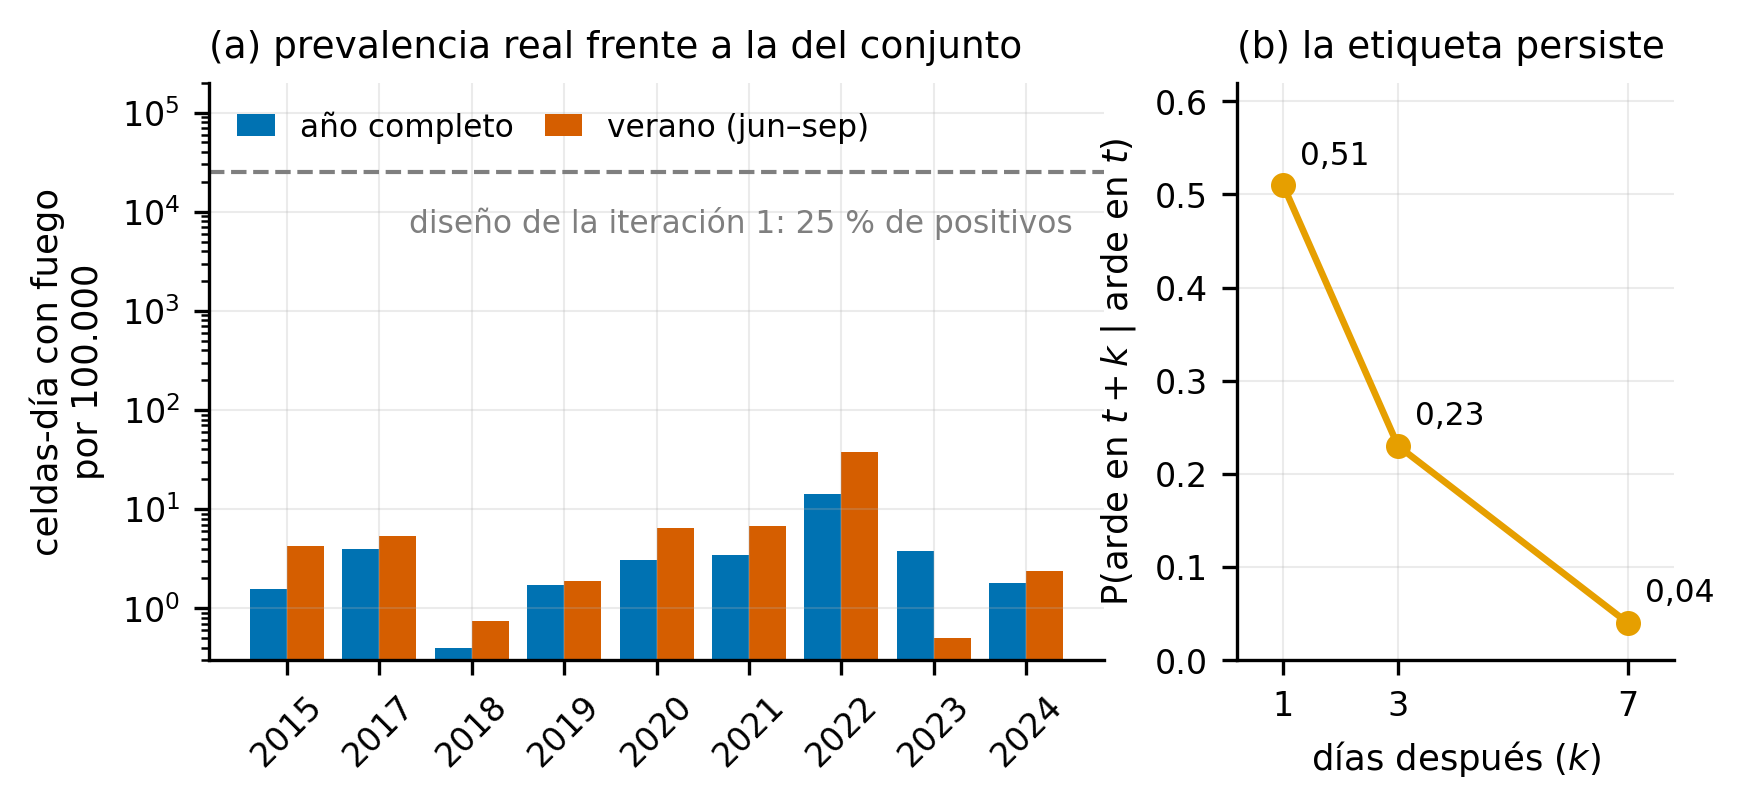
\includegraphics[width=\linewidth]{f7_prevalencia.png}
\caption{Los dos hallazgos del cubo que condicionan el diseño. (a) Prevalencia
real de celdas-día con fuego, en escala logarítmica, frente al 25\,\% de
positivos que tenía el conjunto de la primera iteración. (b) Persistencia de la
etiqueta: la mitad de las celdas que arden un día siguen ardiendo al
siguiente.}
\label{fig:prevalencia}
\end{figure}

La tercera medida del cubo decide cómo se parte. El índice de Moran de las
celdas con EFFIS a un kilómetro es 0,81: a esa escala la etiqueta es sobre todo
perímetro, celdas contiguas del mismo incendio. Partir al azar infla el AUC en
+0,036 frente a partir por bloques de 100\,km, así que todas las particiones
del trabajo son espaciales o temporales y ninguna aleatoria.

\subsection{De la exploración a las variables}

La exploración del conjunto muestreado es la que dio forma a las variables. La
comparación de medianas entre clases (figura~\ref{fig:separacion}) ordena lo que
separa: el FWI absoluto, los días sin lluvia y la precipitación acumulada de 30
días se despegan con claridad, mientras la densidad de población y la distancia
a carreteras tienen exactamente la misma mediana en las dos clases. La
exposición humana explica dónde puede haber ignición a escala de país, pero no
distingue qué día arde una celda concreta.

El hallazgo que más cambió el diseño es que el peligro es relativo a la
climatología del sitio (figura~\ref{fig:normalizacion}). El FWI mediano de los
días de incendio va de 3 en Asturias y Cantabria a 41 en Andalucía: no existe un
umbral absoluto que valga para toda la Península, y un modelo entrenado con FWI
crudo aprende sobre todo a distinguir el norte húmedo del sur seco. El mismo dato
expresado como percentil frente a la climatología de la propia celda se concentra
entre 72 y 92 en las ocho comunidades. De ahí que el FWI entre tres veces
---absoluto, en percentil local y en anomalía tipificada--- y no una.

\begin{figure}[htbp]
\centering
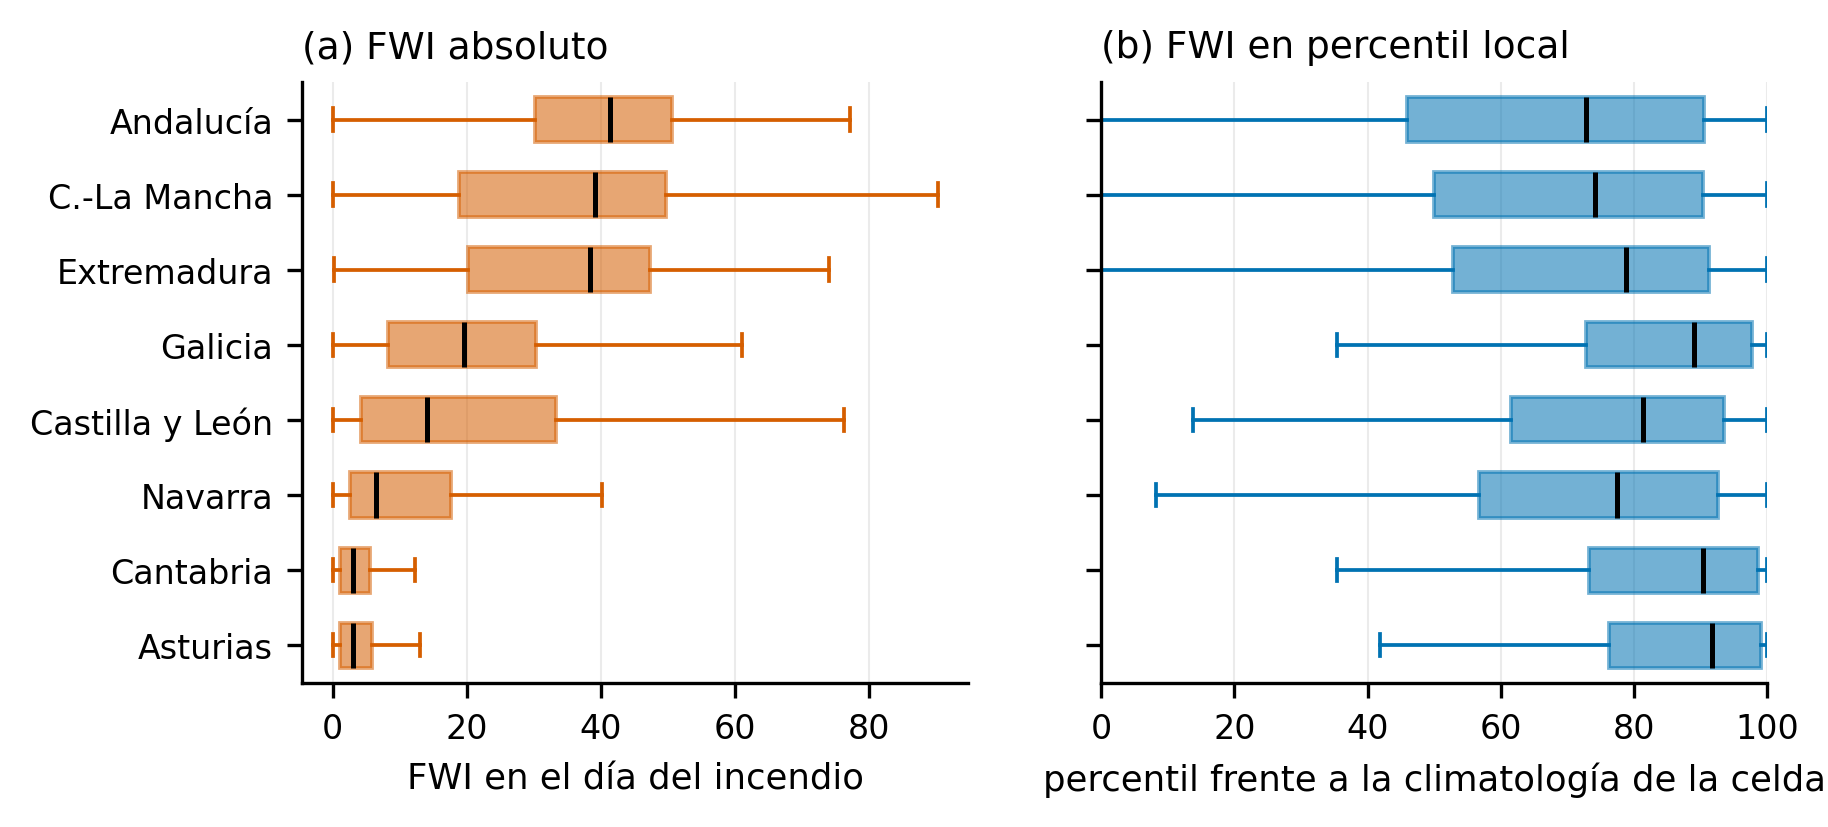
\includegraphics[width=\linewidth]{f8_normalizacion.png}
\caption{El peligro es relativo a la climatología local. Días de incendio del
tramo de entrenamiento, por comunidad autónoma. (a) El FWI absoluto no admite
un umbral común. (b) El percentil local de esos mismos días es alto en todas
partes. Es el argumento de \var{fwi\_pctl\_local}.}
\label{fig:normalizacion}
\end{figure}

La exploración dejó también un aviso para la interpretación posterior. Seis
pares de variables superan $|\rho| = 0{,}8$ ---\var{fwi} con \var{vpd\_max}
(0,86) y con \var{rh\_min} ($-$0,81), \var{fwi\_pctl\_local} con
\var{fwi\_anom\_sigma} (0,96), \var{ndvi} con \var{lai} (0,90)---, de modo que
la importancia por ganancia se reparte entre variables que dicen casi lo mismo.
No se eliminó ninguna, porque los árboles toleran la colinealidad y cada una
aporta en zonas distintas del espacio, pero cualquier lectura de la importancia
tiene que hacerse por bloques y no variable a variable.

\subsection{Del problema al modelo}

El problema se formula como clasificación binaria sobre el par (celda de 1\,km,
día), y en servicio se puntuan las 498.530 celdas del día y se ordenan. La
formulación no dice nada sobre cómo construir el conjunto de entrenamiento, y ahí
es donde se decide de verdad qué pregunta aprende el modelo.

La primera iteración adoptó el diseño habitual en la literatura de
susceptibilidad, caso-control con la celda fija: cada ignición EGIF es un
positivo y sus pseudo-ausencias se sortean en la misma celda en otros días del
mismo bloque temporal, tres por positivo, excluyendo los días con fuego a menos
de 12,5\,km en $\pm$10 días. El clasificador es XGBoost con parada temprana a
100 rondas, hasta 3.000 árboles de profundidad 6, tasa 0,05 y semilla 42, sobre
partición temporal sin solape. Obtiene 0,8906
$[0,8644,\ 0,9136]$ en test 2022 frente al 0,7528 del FWI en percentil, y con
ese número se puso en producción.

La figura~\ref{fig:f3} muestra la primera señal, visible en el propio conjunto
de entrenamiento: el FWI en percentil local separa las clases con holgura
---mediana 84,3 en positivos frente a 47,0 en negativos--- mientras la densidad
de población y la distancia a carreteras tienen exactamente la misma mediana en
las dos. En un diseño de celda fija el positivo y su negativo comparten celda,
así que todo lo estático se cancela por construcción, y el 98,8\,\% de las celdas
del conjunto tenía exactamente un 25\,\% de positivos. El modelo no podía
aprender qué celda es más peligrosa que otra; solo qué día lo es.

\begin{center}
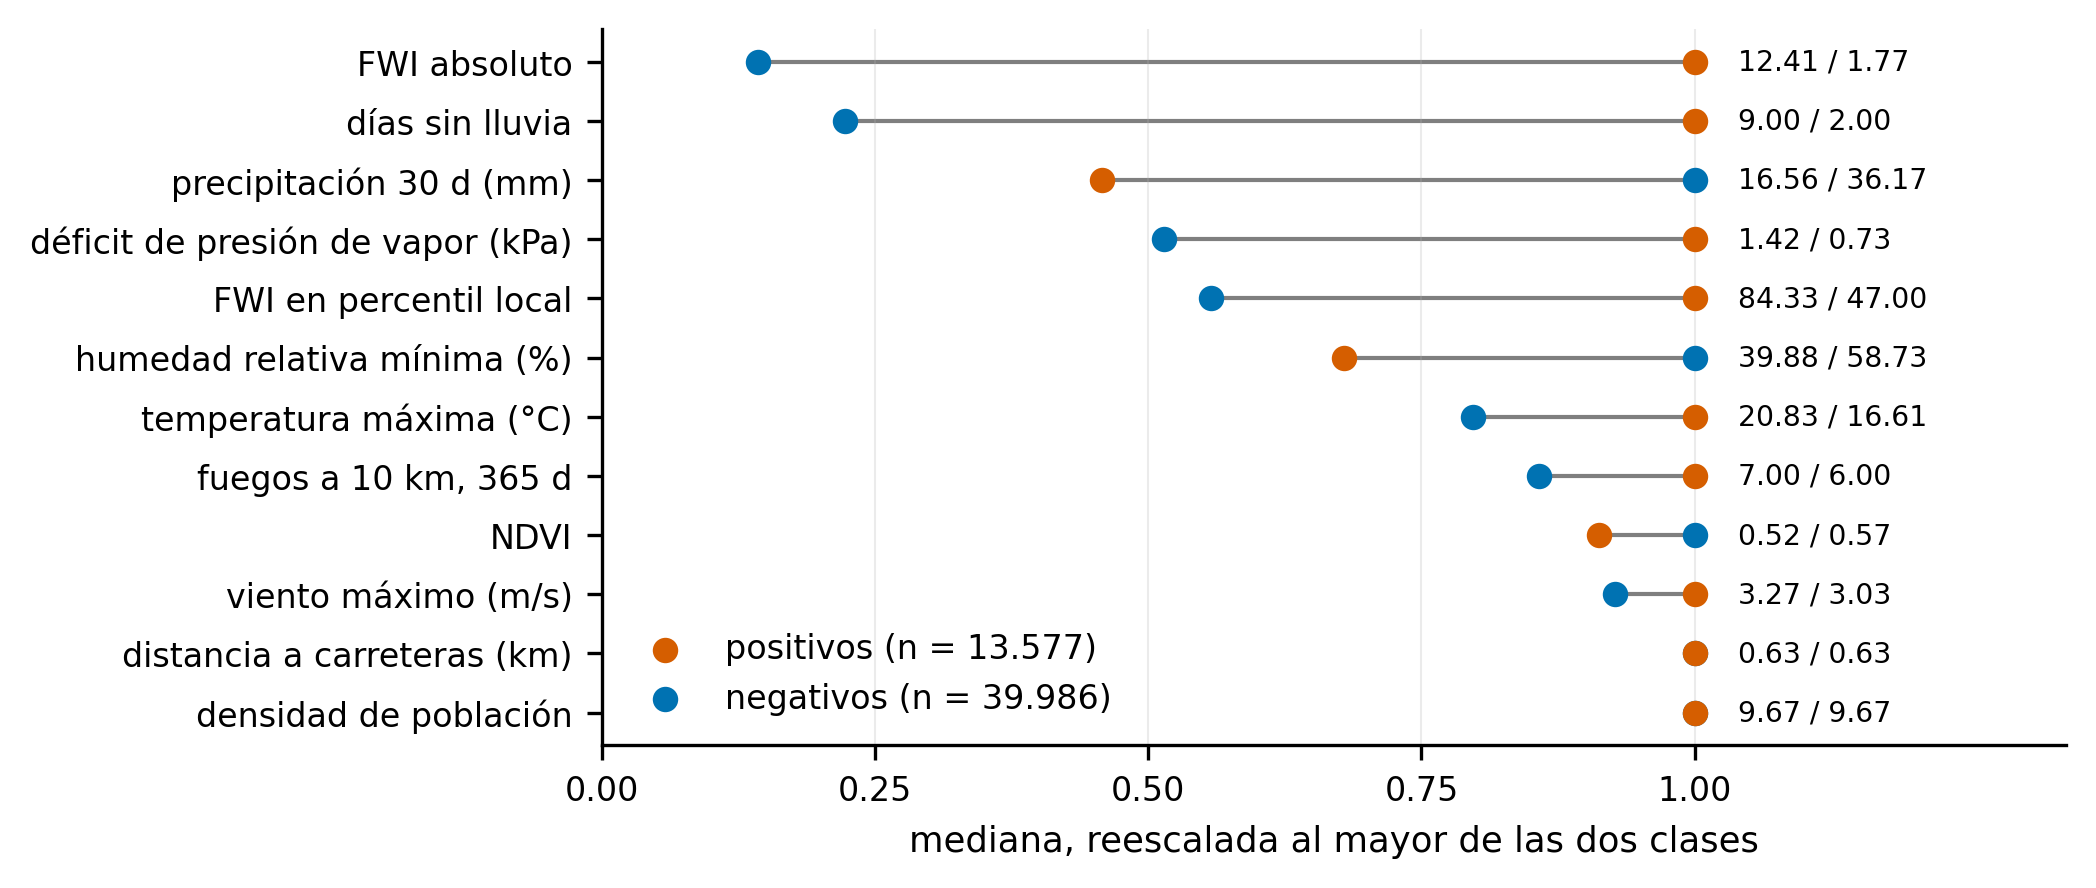
\includegraphics[width=0.88\linewidth]{f3_separacion.png}
\captionof{figure}{Medianas de las variables discriminantes en el conjunto de
entrenamiento de la iteración~1 (53.563 filas, 13.577 positivos), reescaladas al
mayor valor de las dos clases para poder dibujarlas juntas; a la derecha, los
valores sin reescalar (positivos / negativos). En las dos últimas filas los dos
puntos coinciden exactamente: el muestreo con celda fija cancela toda la
información estática del territorio.}
\label{fig:separacion}
\label{fig:f3}
\end{center}

La figura~\ref{fig:f4} cierra el diagnóstico. Dos modelos idénticos en variables
e hiperparámetros, que solo difieren en el diseño de los negativos, resultan
indistinguibles en el banco caso-control de la iteración~1 ---0,922 y 0,916, del
orden del ruido del sorteo--- y se separan 0,082 en el banco operativo, donde
gana el entrenado con negativos del mismo día: la métrica de desarrollo no podía
ver la diferencia que más importaba. Antes se habían agotado las explicaciones más cómodas, todas medidas
y todas negativas: reajustar con más años, rehacer la etiqueta con el EGIF
consolidado ($-0,0012$), entrenar un modelo nativo de estación, servir con
ERA5-Land nativo y congelar las variables de satélite para reproducir el
desajuste con el servicio ($-0,0041$). Ninguna cierra un hueco de veinticinco
centésimas.

\begin{center}
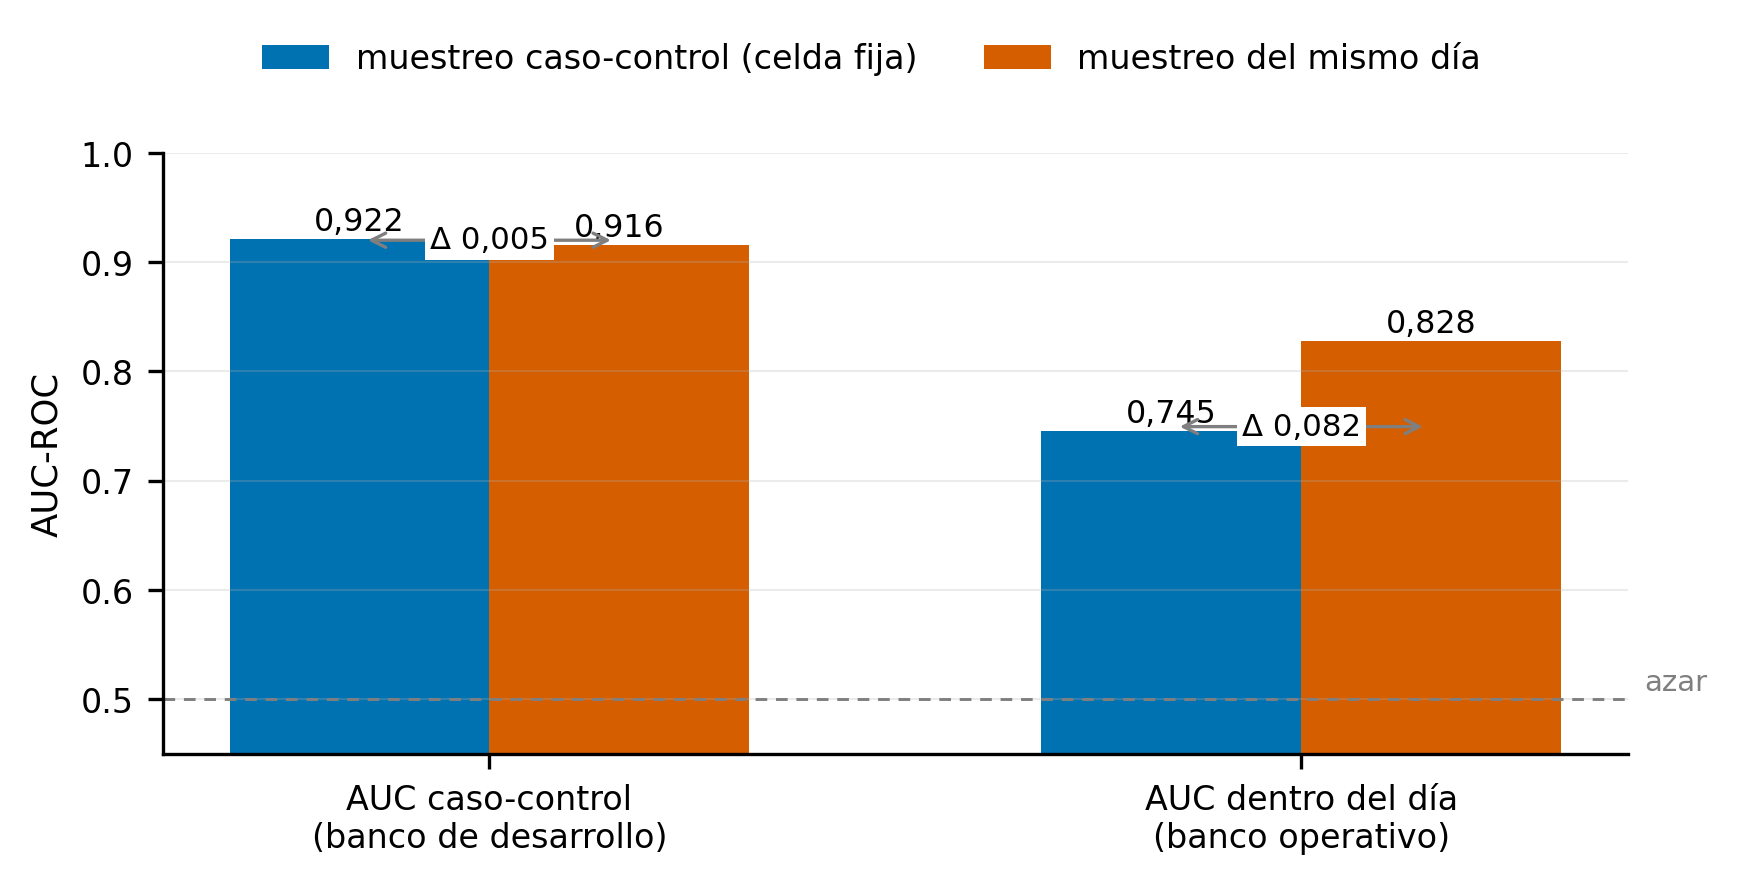
\includegraphics[width=0.8\linewidth]{f4_metrica_ciega.png}
\captionof{figure}{La misma pareja de modelos ---mismas 46 variables, mismos
hiperparámetros, distinto diseño de negativos--- bajo dos métricas. A la
izquierda, AUC en el banco caso-control de cada diseño: indistinguibles. A la
derecha, AUC dentro del día en el banco operativo (test 2020, verdad EGIF): se
separan 0,082. Un buen número en la métrica de desarrollo no garantiza nada
sobre la pregunta operativa si el muestreo no la reproduce.}
\label{fig:f4}
\end{center}

La segunda iteración cambia las dos cosas que el diagnóstico señalaba. La
etiqueta pasa a ser EFFIS, la misma con la que se valida en operación, tomando
como positivo el primer día de cada celda quemada con un tope de 30 por día y
bloque de 100\,km, para que un solo megaincendio no sea la mitad del conjunto; y
los negativos pasan a sortearse el mismo día, en otra celda cualquiera. La
figura~\ref{fig:f2} contrapone los dos
diseños y el banco de evaluación sobre la misma rejilla, y la tabla~\ref{tab:t1}
resume las dos iteraciones. Los hiperparámetros se heredan sin
retoque, de forma deliberada: solo así la diferencia medida es atribuible al
diseño. Se comparan dos arquitecturas ---un modelo único sobre el diseño del
mismo día y la pareja dónde$\times$cuándo del encargo original--- y se ablaciona
el ratio de negativos, heredado como 1:3 sin justificación.

\begin{center}
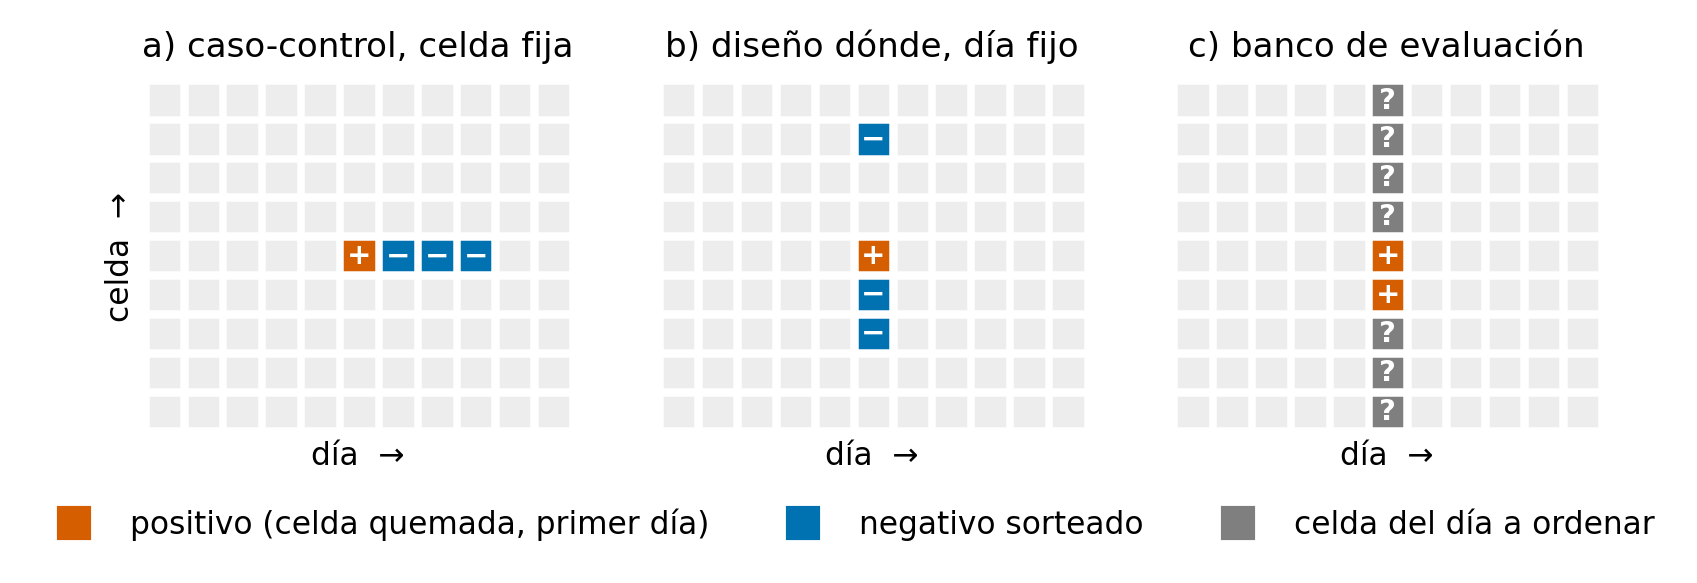
\includegraphics[width=\linewidth]{f2_disenios.png}
\captionof{figure}{Los tres diseños de muestreo sobre la misma rejilla de celdas
y días. En a) el caso-control fija la celda y varía el día, de modo que todo lo
estático se cancela; en b) el diseño del mismo día fija el día y varía la celda,
que es la comparación que hace el usuario del mapa; en c) el banco de evaluación
enfrenta las celdas quemadas del día contra 1.000 celdas sorteadas de ese mismo
día. Los tres se construyen con los mismos datos y dan modelos muy distintos.}
\label{fig:f2}
\end{center}

Sobre el control de la fuga de información conviene ser explícito, porque hubo
una. Además de la regla de ventanas estrictas, se auditó cada variable comparando
su desplazamiento en la celda que arde el día $D$ contra un anillo de control.
Tres de las 46 ---NDVI, temperatura de superficie y humedad
superficial--- resultaron concurrentes: el satélite ya ve la firma del incendio el
mismo día. La prueba está automatizada en
\var{dos\_24\_auditoria\_fugas.py} y acompaña a esta memoria en el repositorio,
igual que la comprobación de desfase de \var{dos\_23\_vispera.py}.
Pesan el 4,6\,\% de la importancia del modelo único y no sesgan la
comparación, porque ambas iteraciones comparten receta, pero inflan los valores
absolutos de toda evaluación del mismo día. Se detectó además que la interfaz de
FIRMS cuenta los cinco días hacia adelante desde la fecha pedida y no hacia
atrás, con lo que el mapa retrospectivo del día $D$ llevaba dentro los focos del
propio incendio; entrenamiento y producción estaban limpios, y la evaluación
retrospectiva se relanzó entera. El arreglo refuerza la conclusión: la ventaja
del rediseño pasa de $+0,037$, rozando el cero, a $+0,105$.

\begin{center}\footnotesize
\begin{tabular}{@{}L{2.9cm}L{6.2cm}L{6.2cm}@{}}
\toprule
 & \textbf{Iteración 1 (grupo de control)} & \textbf{Iteración 2 (rediseño)} \\
\midrule
Etiqueta & EGIF, ignición puntual, 2015--2020 & EFFIS \var{is\_fire}, celda quemada $\geq$5\,ha, primer día \\
Negativos & misma celda, otro día; 1:3; buffer 12,5\,km y $\pm$10 días & mismo día, otra celda; ratio ablacionado de 1:3 a 1:100 \\
Partición & train 2015--2020 / val 2021 / test 2022 & train 2015--2022 / val 2023 / test 2024 / externo 2026 \\
Variables & 46 & 46 (las mismas) \\
Métrica de desarrollo & AUC-ROC caso-control 0,8906 $[0,8644,\ 0,9136]$ & AUC-PR en validación de 0,950 (1:3) a 0,737 (1:100) \\
Métrica operativa (2026) & AUC dentro del día 0,647 & 0,752 (1:3) y 0,759 (1:10) \\
\bottomrule
\end{tabular}
\captionof{table}{Las dos iteraciones lado a lado. La comparación es del diseño
del conjunto de entrenamiento: fuentes, variables, hiperparámetros y semillas son
idénticos, y la partición cambia solo porque EFFIS cubre años que EGIF no cubre.}
\label{tab:t1}
\end{center}

\subsection{Evaluación}

La métrica principal es el AUC-ROC calculado dentro de cada día: para cada día
con al menos un positivo se enfrentan las celdas quemadas de ese día contra 1.000
celdas sorteadas del mismo día, y se promedia sobre días. Reproduce la decisión
operativa ---ordenar las celdas de hoy, no comparar hoy con otro día---, mientras
que un AUC global premia sobre todo acertar qué días son peligrosos, que es
información que el usuario ya tiene. Y el desbalanceo obliga: con una prevalencia
del orden de cinco celdas por cada 100.000 y día, toda métrica de umbral fijo es
inutilizable y el AUC-PR global queda dominado por los pocos días de
megaincendio. Como complemento se
reportan el lift del decil superior, el percentil ---también ponderado por
hectáreas--- en que cae la celda quemada, y la cobertura de superficie quemada
dentro del 2\,\% mejor puntuado. Los intervalos salen de un bootstrap de 2.000
remuestreos de días completos, nunca de celdas.

Las líneas base son el FWI en percentil local, un mapa estático de
susceptibilidad y, sobre todo, el modelo de producción, que es lo que hoy se
sirve. En el test
interno de 2024 la ventaja del modelo único todavía no es concluyente: 0,809
frente a 0,792, intervalo $[-0,024,\ +0,063]$, con el FWI en 0,636 y la pareja
dónde$\times$cuándo en 0,762. Es la temporada 2026, con 74 días,
4.843 celdas quemadas y 260.753 hectáreas, la que resuelve: producción 0,647,
modelo único 0,752 ($+0,105$ $[+0,067,\ +0,146]$, 70\,\% de días ganados) y el
mismo modelo con ratio 1:10 en 0,759 ($+0,112$ $[+0,074,\ +0,151]$, 76\,\%). La
pareja queda en 0,705. La figura~\ref{fig:f5} muestra la serie y la trayectoria
del intervalo.

\begin{center}
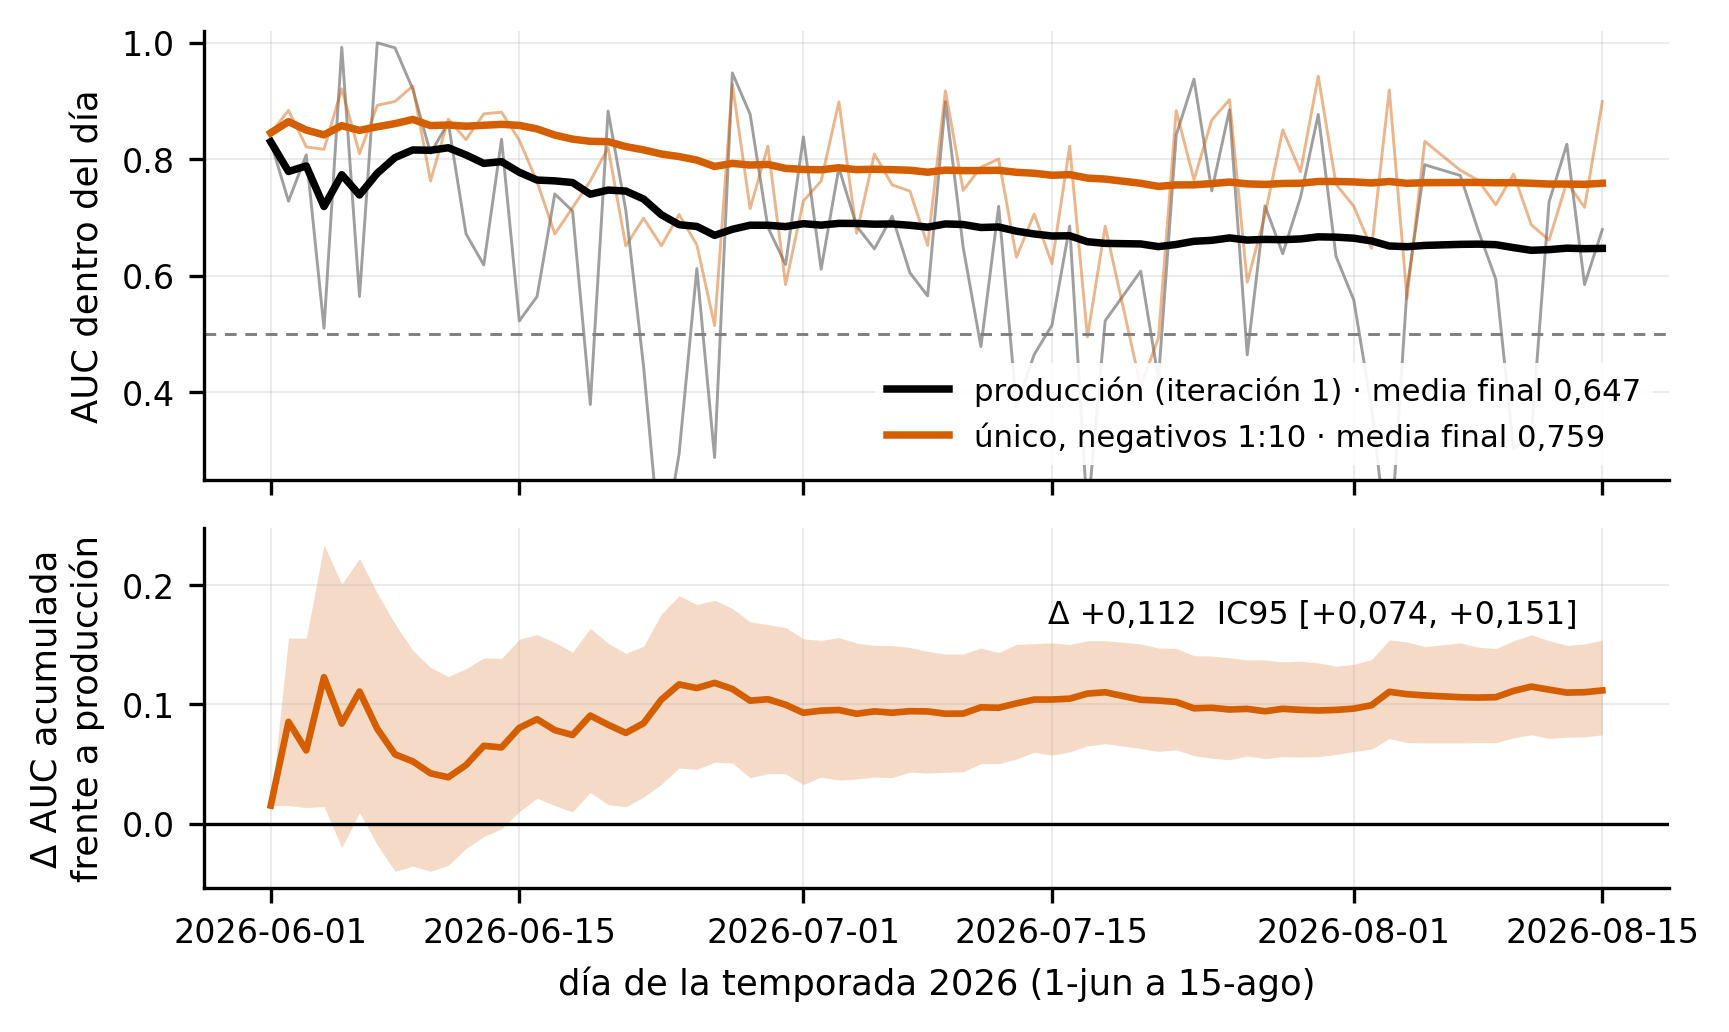
\includegraphics[width=0.9\linewidth]{f5_temporada2026.png}
\captionof{figure}{Temporada 2026, del 1 de junio al 15 de agosto. Arriba, AUC
dentro del día: la línea fina es el valor diario ---ruidoso, porque un día con
tres celdas quemadas no dice nada--- y la gruesa su media acumulada. Abajo, la
diferencia pareada acumulada contra producción con su intervalo al 95\,\% por
bootstrap de días. El número que se defiende es el del último día, fijado de
antemano al cierre de la temporada; leer la banda cada día y cantar victoria el
primero en que despega del cero sería \emph{peeking} sobre 74 miradas.}
\label{fig:f5}
\end{center}

Las ablaciones acotan de dónde sale la ventaja. El ratio de negativos tiene un
óptimo interior: la escalera 1:3, 1:10, 1:30, 1:60 y 1:100 da en 2026 valores de
0,748, 0,759, 0,753, 0,748 y 0,745. Esa ganancia es del orden del ruido de volver
a sortear los negativos con la misma receta, medido en 0,004; lo que sí mejora es
el fuego grande, con el percentil ponderado por hectáreas subiendo de 76,2 en
producción a 79,8 en el modelo único y 81,9 en la variante 1:10. Entrenar solo con los meses de verano empeora ($-0,028$), y añadir
una capa que apague el riesgo en lo ya quemado también ($-0,021$), coherente con
la etiqueta: EFFIS marca días ardiendo y penaliza bajar el riesgo de un perímetro
activo. Los focos FIRMS aportan menos de lo que se creía, $+0,036$, sin llegar a
la punta del ranking.

El análisis de error se resume en la figura~\ref{fig:f6}. El modelo único
concentra el 29,2\,\% de su importancia en una sola variable, la densidad
histórica de incendios a 10\,km en el mismo mes, seguida de los usos del suelo
CORINE (14,3\,\%) y la pendiente (5,8\,\%); producción reparte su peso sobre la
meteorología, con el 20,5\,\% en la anomalía tipificada del FWI. Al cambiar el
muestreo, el modelo deja de aprender el cuándo y empieza a aprender el dónde. El
precio está en el panel derecho:
el modelo único pierde muy poco acierto cuando se le desplaza el mapa uno, dos o
tres días respecto al día del fuego, mientras producción pierde de forma clara.
Un mapa que no pierde nada al alejarse del suceso se apoya en lo persistente
---el territorio--- y no en la ignición concreta: ahí está el límite del sistema
y el sitio por donde tiene que crecer. La misma comprobación, leída al revés, es
la que destapó la fuga de FIRMS: si el acierto no decae al alejar el predictor
del suceso, algo está viendo el suceso.

\begin{center}
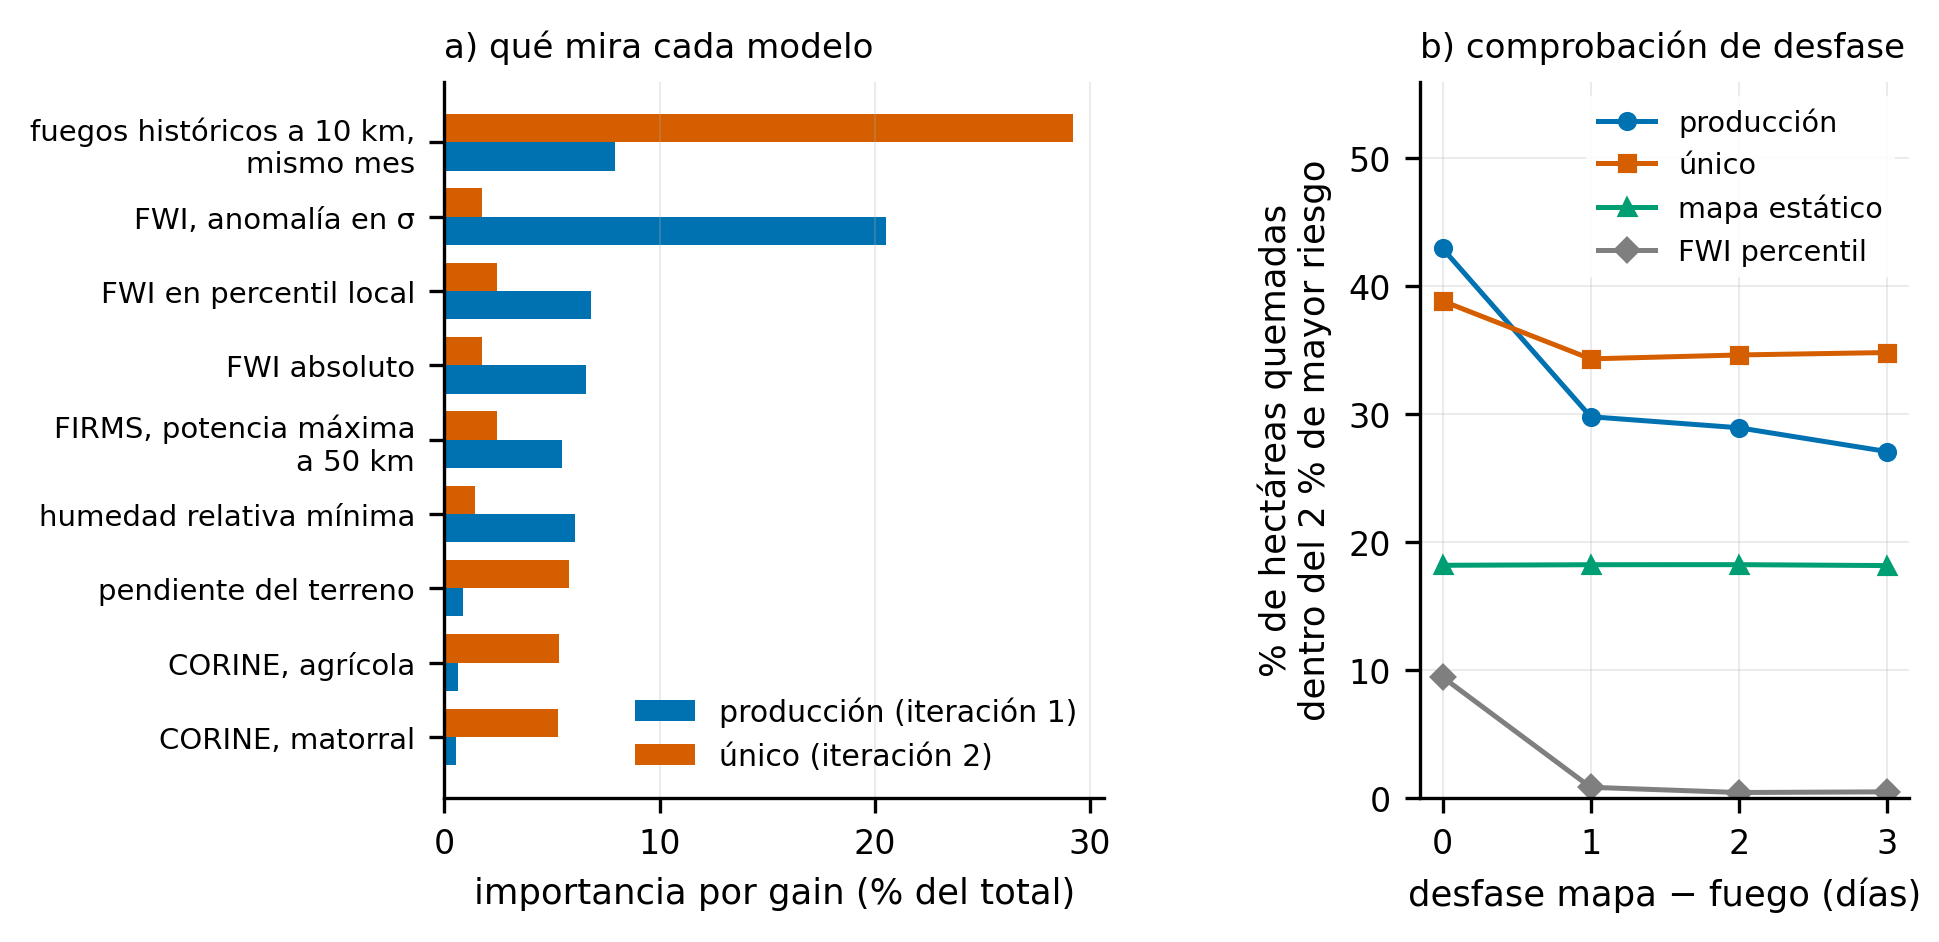
\includegraphics[width=\linewidth]{f6_donde_mira.png}
\captionof{figure}{Izquierda: importancia por \emph{gain} de los dos modelos
sobre las nueve variables más pesadas. Derecha: porcentaje de hectáreas quemadas
del día que caen dentro del 2\,\% de celdas de mayor riesgo, según los días de
desfase entre el mapa y el fuego. El mapa estático es plano por construcción y el
FWI se desploma; entre esos dos extremos, cuanto más plana es la curva, más se
apoya el modelo en el territorio y menos en el día concreto.}
\label{fig:f6}
\end{center}

\subsection{Limitaciones y trabajo posterior}

La limitación de fondo es que la ventaja se demuestra en evaluación
retrospectiva, con reanálisis meteorológico para todos los modelos: es un cara a
cara limpio, pero una cota superior de lo que dará la operación, donde se trabaja
con previsión. La única comparación sin retrovisor para nadie son 19 días de julio y agosto de 2026 contra el ranking sellado
que se público ese mismo día: por estación meteorológica el modelo único obtiene
0,605 frente a 0,568 y gana 14 de los 19 días, pero con intervalo
$[-0,020,\ +0,085]$; por celda la diferencia sí es concluyente, 0,755 frente a
0,669 $[+0,022,\ +0,156]$.

Tres limitaciones más, todas asumidas. Las variables concurrentes ya mencionadas
inflan los valores absolutos de toda evaluación del mismo día, aunque no la
comparación. El modelo se entrenó con una ventana de focos FIRMS de siete días
mientras la tubería de servicio pedía cinco; corregirlo aporta $+0,003$, ruido,
pero es un desajuste real que estuvo sin detectar. Y el repositorio que acompaña
a esta memoria todavía no incluye un fichero de entorno con las versiones de las
dependencias, de modo que ninguna cifra es reejecutable tal cual por un tercero:
es el hueco más grave que queda abierto. Tampoco hay curva de
precisión-exhaustividad ni análisis de calibración de la segunda iteración, que
sí existen para la primera.

Ordenadas por relación entre valor y esfuerzo, las acciones siguientes son
cuatro. La primera, cerrar el fichero de entorno y la ejecución de demostración:
trabajo de horas, y lo que separa un repositorio legible de uno reproducible. La
segunda, servir la variante con ratio 1:10, que ya está
entrenada, publicada y recogida por los tres jueces en operación. La tercera,
atacar el radio de 50\,km de las variables FIRMS, la hipótesis viva para explicar
por qué los focos activos no ayudan en la punta del ranking: un radio tan grueso
arrastra la puntuación hacia lo que ya ha ardido en lugar de hacia la ignición
nueva. La cuarta, ya como trabajo futuro, entrenar sobre previsiones en lugar de
reanálisis, que es la única forma de cerrar la distancia entre la cifra
retrospectiva y la operativa. Las tres primeras están preparadas en el
repositorio; la cuarta no. El veredicto acumulado de los tres jueces se cierra a
mediados de septiembre de 2026 y es el que decide.

\end{document}
